% This LaTeX was auto-generated from MATLAB code.
% To make changes, update the MATLAB code and export to LaTeX again.

\documentclass{article}

\usepackage[utf8]{inputenc}
\usepackage[T1]{fontenc}
\usepackage{lmodern}
\usepackage{graphicx}
\usepackage{color}
\usepackage{hyperref}
\usepackage{amsmath}
\usepackage{amsfonts}
\usepackage{epstopdf}
\usepackage[table]{xcolor}
\usepackage{matlab}

\sloppy
\epstopdfsetup{outdir=./}
\graphicspath{ {./polynomial_interpolation_images/} }

\begin{document}

\matlabtitle{Polynomial interpolation}

\begin{par}
\begin{flushleft}
Funzione seno. Genera dei punti rumorosi che seguono l'andamento del seno e poi determina il polinomio che passa per i punti. Grafica anche gli errori di Learning e Testing e individua il minimo
\end{flushleft}
\end{par}

\begin{matlabcode}
% cleaning
clc
clear

% funzione seno
sen = @(x) sin(2*pi*x);

% genero vettori
x = linspace(0,1,100);
y = sen(x);

% plotto funzione seno
figure;
plot(x,y)
xlabel("x")
ylabel("y")
legend("sin(2\pix)")
\end{matlabcode}


\begin{par}
\begin{flushleft}
In general, you can generate \texttt{N} random numbers in the interval (a,b) with the formula \texttt{r = a + (b-a).*rand(N,1)}.
\end{flushleft}
\end{par}

\begin{matlabcode}
% genero set di learning
n_lrn = 10;
x_lrn = linspace(0,1,n_lrn)
eps = 0.15;
y_lrn = sin(2*pi*x_lrn)
y_lrn = y_lrn + (-eps + (2.*eps).*rand(n_lrn,1))'

figure
plot(x,y)
hold on
plot(x_lrn,y_lrn,"o")
legend("sin(2\pix)","data")
xlabel("x")
ylabel("y")
hold off
\end{matlabcode}


\begin{matlabcode}
% genero matrice di Vandermonde
V = fliplr(vander(x_lrn))
\end{matlabcode}

\begin{par}
\begin{flushleft}
Risolvo il sistema lineare $y=\alpha V$ dove $\alpha$ sono i coefficienti del polinomio cercato: $y=\alpha_1 +\alpha_2 x_1 +\alpha_3 x_2^2 +...$
\end{flushleft}
\end{par}

\begin{par}
\begin{flushleft}
Alla luce della forma matriciale, i coefficienti $\alpha$ eseguendo il prodotto righe per colonna tra l'inversa della matrice di Vandermonde e il vettore colonna y
\end{flushleft}
\end{par}

\begin{matlabcode}
% determino i coefficienti
a = pinv(V)*(y_lrn')

% ottengo il polinomio
poly = @(x_lrn) x_lrn.^(0:n_lrn-1)*a; % prod riga per colonna

z = zeros(1,100);
for i=1:100
    z(i) = poly(x(i));
end
\end{matlabcode}


\begin{matlabcode}
figure;
plot(x,z,"r")
hold on
plot(x_lrn,y_lrn,'ob')
plot(x,y,"g")
hold off
legend("polynomial fit", "data", "sin(2\pix)")
xlabel("x")
ylabel("y")
ylim([-1.5 1.5])
xlim([0 1])
\end{matlabcode}
\begin{center}
\includegraphics[width=\maxwidth{56.196688409433015em}]{figure_0.eps}
\end{center}


\begin{matlabcode}

% test
% figure;
% plot(x,repelem(a(1),length(x)))
% hold on
% plot(x,(a(1) + a(2).*x))
% plot(x,(a(1) + a(2).*x + a(3).*x.^2))
% hold off
% ylim([-1.5 1.5])
% xlim([0 1])

% plot M = 0
figure;
plot(x,repelem(a(1),length(x)),"r")
hold on
plot(x_lrn,y_lrn,'ob')
plot(x,y,"g")
hold off
legend("polynomial fit", "data", "sin(2\pix)")
xlabel("x")
ylabel("y")
ylim([-1.5 1.5])
xlim([0 1])
title("M=0")
\end{matlabcode}
\begin{center}
\includegraphics[width=\maxwidth{56.196688409433015em}]{figure_1.eps}
\end{center}
\begin{matlabcode}

% plot M = 1
figure;
plot(x,(a(1)+a(2).*x),"r")
hold on
plot(x_lrn,y_lrn,'ob')
plot(x,y,"g")
hold off
legend("polynomial fit", "data", "sin(2\pix)")
xlabel("x")
ylabel("y")
ylim([-1.5 1.5])
xlim([0 1])
title("M=1")
\end{matlabcode}
\begin{center}
\includegraphics[width=\maxwidth{56.196688409433015em}]{figure_2.eps}
\end{center}
\begin{matlabcode}

% plot M = 3
figure;
plot(x,(a(1) + (a(2).*x) + a(3).*x.^2 + a(4).*x.^3),"r")
hold on
plot(x_lrn,y_lrn,'ob')
plot(x,y,"g")
hold off
legend("polynomial fit", "data", "sin(2\pix)")
xlabel("x")
ylabel("y")
ylim([-1.5 1.5])
xlim([0 1])
title("M=3")
\end{matlabcode}
\begin{center}
\includegraphics[width=\maxwidth{56.196688409433015em}]{figure_3.eps}
\end{center}
\begin{matlabcode}

\end{matlabcode}
\begin{center}
\includegraphics[width=\maxwidth{56.196688409433015em}]{figure_4.eps}
\end{center}

\end{document}
